\section{Data Preprocessing}\label{data_preprocessing}

Data preprocessing is a vital step in the data mining process, particularly in the context of deep learning for image classification. This step involves techniques such as image augmentation, affine transformations, and resizing, which are essential for enhancing model performance. For this project, preprocessing is applied to the provided dataset (dataset\_19) to ensure it is suitable for the brain tumor classification task. The specific steps involved in the preprocessing of this dataset are outlined below.

\subsection{Image Cropping and Enhancement}\label{image_cropping_enhancement}

A fundamental step in our preprocessing workflow is the cropping and enhancement of images to focus exclusively on the brain, effectively eliminating irrelevant background elements. The following sequence outlines the improved procedures:

\textbf{Conversion and Blurring:} The images are first converted to grayscale to diminish computational complexity and concentrate on structural attributes without the influence of color. This is immediately followed by the application of a Gaussian blur with a $3 \times 3$
 kernel to soften the image noise, which facilitates more reliable edge detection in the subsequent stages.

\textbf{Thresholding and Morphology:} Using a threshold value of 45, adaptive thresholding converts the grayscale images into binary images to segregate the brain tissue from the background. The binary images then undergo a series of erosions and dilations—two iterations each—to eradicate small noise regions and clarify the brain's structural outline.

\textbf{Contour Detection and Cropping:} Contours are extracted from the thresholded image using external retrieval mode, with the largest contour presumed to represent the brain's boundary. This contour's extreme points (left, right, top, bottom) are determined, and the image is cropped to this bounding rectangle, expanded by a configurable pixel margin, to ensure the brain is isolated without clipping.

\textbf{Further Processing:} Each cropped image is then converted back to grayscale, enhanced using bilateral filtering to further reduce noise and sharpen edges, and mapped to a 'bone' color scheme to improve visual contrast and detail. Images are resized to $224 \times 224$
 pixels for uniformity and computational efficiency.

These steps, as shown in Figure \ref{fig:image_cropping}, not only decrease the computational load but also significantly enhance the clarity and focus on essential features for more effective classification.

\begin{figure}[H]
  \begin{center}
    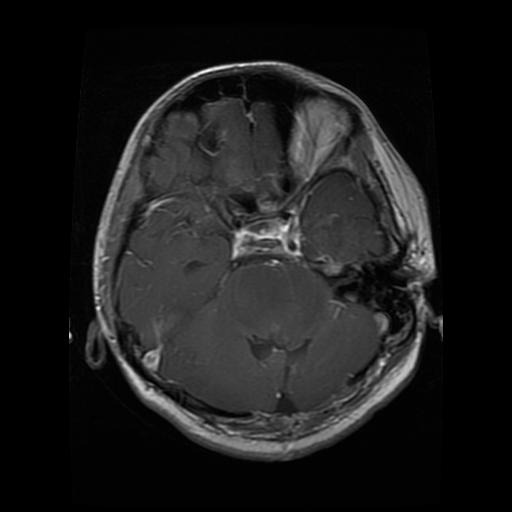
\includegraphics[width=0.3\textwidth]{Exploration/Te-gl_0010.jpg}
    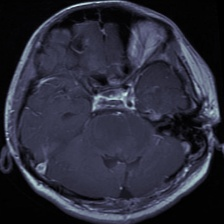
\includegraphics[width=0.3\textwidth]{Exploration/Te-gl_0010_preprocessed.jpg}
  \end{center}
  \caption{Cropping the MRI image along its contour.}\label{fig:image_cropping}
\end{figure}



\subsection{Data Augmentation}\label{data_augmentation}

Following the initial preprocessing steps, we apply image augmentation techniques using the \texttt{ImageDataGenerator} class from the Keras library. Each model is fine-tuned with a subset of these techniques, which include horizontal flips, random rotations, and normalization. As referenced in \cite{nalepa_data_2019}, certain affine augmentations can be advantageous for brain tumor classification tasks. However, it is crucial to note that some augmentations, such as vertical flips, may be detrimental due to the potential misrepresentation of tumor locations.

Importantly, these augmentation techniques are applied exclusively to the training dataset, while the validation dataset remains unaltered. This strategy ensures that the model encounters a diverse array of augmented images during training, thereby enhancing its generalization capabilities without compromising the integrity of the evaluation process.

For each model evaluation, we provide a detailed commentary on the preprocessing and augmentation techniques employed, along with the rationale behind their selection. This comprehensive analysis elucidates how these techniques contribute to the overall performance and generalization capabilities of the models.

\subsection{Data Splitting}\label{data_splitting}
After preprocessing and augmentation, the dataset is divided into training and validation sets, with the training set comprising 80\% of the data and the validation set the remaining 20\%. This distribution allows the model to be trained extensively while also being evaluated on a separate set of data to assess its performance, as depicted in Figure \ref{fig:data_split}.

\begin{figure}[H]
  \begin{center}
    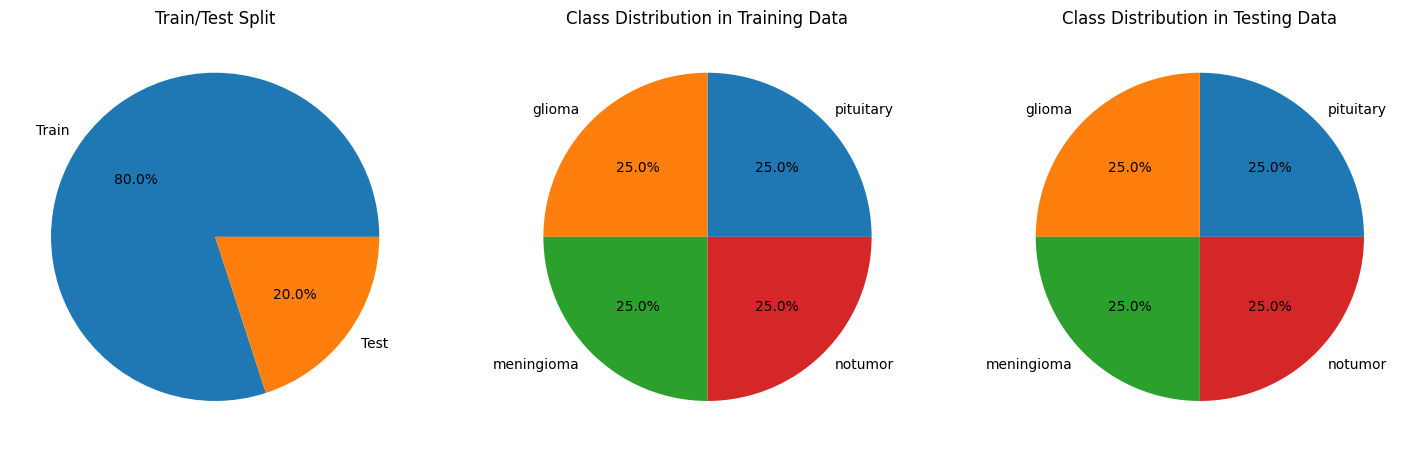
\includegraphics[width=0.95\textwidth]{Exploration/data_split.png}
  \end{center}
  \caption{Splitting the dataset into training and validation sets.}\label{fig:data_split}
\end{figure}


\subsection{Summary and Justifications}

Given the relatively small size of dataset\_19 (480 images in total), data augmentation is crucial for enhancing the dataset's variability and improving the model's generalization capabilities. Flipping images horizontally is justified based on the anatomical symmetry of the brain's hemispheres, allowing for effective augmentation without misrepresenting tumor locations \cite{nalepa_data_2019}. This technique increases the diversity of the training data, which is particularly important given the limited size of the dataset compared to larger datasets, such as those used in the BraTS competition.

Similarly, random rotations are applied since brain images can be rotated in various directions, further increasing the dataset's variability and aiding in model training. The augmentation strategies, including horizontal flipping and random rotations, are essential for compensating for the smaller dataset size by exposing the model to a wider variety of image orientations and perspectives. This approach helps create a more robust model capable of accurately classifying brain tumors despite the limited amount of original training data.

